% Options for packages loaded elsewhere
\PassOptionsToPackage{unicode}{hyperref}
\PassOptionsToPackage{hyphens}{url}
\PassOptionsToPackage{dvipsnames,svgnames,x11names}{xcolor}
%
\documentclass[
]{article}
\usepackage{amsmath,amssymb}
\usepackage{iftex}
\ifPDFTeX
  \usepackage[T1]{fontenc}
  \usepackage[utf8]{inputenc}
  \usepackage{textcomp} % provide euro and other symbols
\else % if luatex or xetex
  \usepackage{unicode-math} % this also loads fontspec
  \defaultfontfeatures{Scale=MatchLowercase}
  \defaultfontfeatures[\rmfamily]{Ligatures=TeX,Scale=1}
\fi
\usepackage{lmodern}
\ifPDFTeX\else
  % xetex/luatex font selection
\fi
% Use upquote if available, for straight quotes in verbatim environments
\IfFileExists{upquote.sty}{\usepackage{upquote}}{}
\IfFileExists{microtype.sty}{% use microtype if available
  \usepackage[]{microtype}
  \UseMicrotypeSet[protrusion]{basicmath} % disable protrusion for tt fonts
}{}
\makeatletter
\@ifundefined{KOMAClassName}{% if non-KOMA class
  \IfFileExists{parskip.sty}{%
    \usepackage{parskip}
  }{% else
    \setlength{\parindent}{0pt}
    \setlength{\parskip}{6pt plus 2pt minus 1pt}}
}{% if KOMA class
  \KOMAoptions{parskip=half}}
\makeatother
\usepackage{xcolor}
\usepackage[margin=1in]{geometry}
\usepackage{color}
\usepackage{fancyvrb}
\newcommand{\VerbBar}{|}
\newcommand{\VERB}{\Verb[commandchars=\\\{\}]}
\DefineVerbatimEnvironment{Highlighting}{Verbatim}{commandchars=\\\{\}}
% Add ',fontsize=\small' for more characters per line
\usepackage{framed}
\definecolor{shadecolor}{RGB}{248,248,248}
\newenvironment{Shaded}{\begin{snugshade}}{\end{snugshade}}
\newcommand{\AlertTok}[1]{\textcolor[rgb]{0.94,0.16,0.16}{#1}}
\newcommand{\AnnotationTok}[1]{\textcolor[rgb]{0.56,0.35,0.01}{\textbf{\textit{#1}}}}
\newcommand{\AttributeTok}[1]{\textcolor[rgb]{0.13,0.29,0.53}{#1}}
\newcommand{\BaseNTok}[1]{\textcolor[rgb]{0.00,0.00,0.81}{#1}}
\newcommand{\BuiltInTok}[1]{#1}
\newcommand{\CharTok}[1]{\textcolor[rgb]{0.31,0.60,0.02}{#1}}
\newcommand{\CommentTok}[1]{\textcolor[rgb]{0.56,0.35,0.01}{\textit{#1}}}
\newcommand{\CommentVarTok}[1]{\textcolor[rgb]{0.56,0.35,0.01}{\textbf{\textit{#1}}}}
\newcommand{\ConstantTok}[1]{\textcolor[rgb]{0.56,0.35,0.01}{#1}}
\newcommand{\ControlFlowTok}[1]{\textcolor[rgb]{0.13,0.29,0.53}{\textbf{#1}}}
\newcommand{\DataTypeTok}[1]{\textcolor[rgb]{0.13,0.29,0.53}{#1}}
\newcommand{\DecValTok}[1]{\textcolor[rgb]{0.00,0.00,0.81}{#1}}
\newcommand{\DocumentationTok}[1]{\textcolor[rgb]{0.56,0.35,0.01}{\textbf{\textit{#1}}}}
\newcommand{\ErrorTok}[1]{\textcolor[rgb]{0.64,0.00,0.00}{\textbf{#1}}}
\newcommand{\ExtensionTok}[1]{#1}
\newcommand{\FloatTok}[1]{\textcolor[rgb]{0.00,0.00,0.81}{#1}}
\newcommand{\FunctionTok}[1]{\textcolor[rgb]{0.13,0.29,0.53}{\textbf{#1}}}
\newcommand{\ImportTok}[1]{#1}
\newcommand{\InformationTok}[1]{\textcolor[rgb]{0.56,0.35,0.01}{\textbf{\textit{#1}}}}
\newcommand{\KeywordTok}[1]{\textcolor[rgb]{0.13,0.29,0.53}{\textbf{#1}}}
\newcommand{\NormalTok}[1]{#1}
\newcommand{\OperatorTok}[1]{\textcolor[rgb]{0.81,0.36,0.00}{\textbf{#1}}}
\newcommand{\OtherTok}[1]{\textcolor[rgb]{0.56,0.35,0.01}{#1}}
\newcommand{\PreprocessorTok}[1]{\textcolor[rgb]{0.56,0.35,0.01}{\textit{#1}}}
\newcommand{\RegionMarkerTok}[1]{#1}
\newcommand{\SpecialCharTok}[1]{\textcolor[rgb]{0.81,0.36,0.00}{\textbf{#1}}}
\newcommand{\SpecialStringTok}[1]{\textcolor[rgb]{0.31,0.60,0.02}{#1}}
\newcommand{\StringTok}[1]{\textcolor[rgb]{0.31,0.60,0.02}{#1}}
\newcommand{\VariableTok}[1]{\textcolor[rgb]{0.00,0.00,0.00}{#1}}
\newcommand{\VerbatimStringTok}[1]{\textcolor[rgb]{0.31,0.60,0.02}{#1}}
\newcommand{\WarningTok}[1]{\textcolor[rgb]{0.56,0.35,0.01}{\textbf{\textit{#1}}}}
\usepackage{longtable,booktabs,array}
\usepackage{calc} % for calculating minipage widths
% Correct order of tables after \paragraph or \subparagraph
\usepackage{etoolbox}
\makeatletter
\patchcmd\longtable{\par}{\if@noskipsec\mbox{}\fi\par}{}{}
\makeatother
% Allow footnotes in longtable head/foot
\IfFileExists{footnotehyper.sty}{\usepackage{footnotehyper}}{\usepackage{footnote}}
\makesavenoteenv{longtable}
\usepackage{graphicx}
\makeatletter
\def\maxwidth{\ifdim\Gin@nat@width>\linewidth\linewidth\else\Gin@nat@width\fi}
\def\maxheight{\ifdim\Gin@nat@height>\textheight\textheight\else\Gin@nat@height\fi}
\makeatother
% Scale images if necessary, so that they will not overflow the page
% margins by default, and it is still possible to overwrite the defaults
% using explicit options in \includegraphics[width, height, ...]{}
\setkeys{Gin}{width=\maxwidth,height=\maxheight,keepaspectratio}
% Set default figure placement to htbp
\makeatletter
\def\fps@figure{htbp}
\makeatother
\setlength{\emergencystretch}{3em} % prevent overfull lines
\providecommand{\tightlist}{%
  \setlength{\itemsep}{0pt}\setlength{\parskip}{0pt}}
\setcounter{secnumdepth}{-\maxdimen} % remove section numbering
\newlength{\cslhangindent}
\setlength{\cslhangindent}{1.5em}
\newlength{\csllabelwidth}
\setlength{\csllabelwidth}{3em}
\newlength{\cslentryspacingunit} % times entry-spacing
\setlength{\cslentryspacingunit}{\parskip}
\newenvironment{CSLReferences}[2] % #1 hanging-ident, #2 entry spacing
 {% don't indent paragraphs
  \setlength{\parindent}{0pt}
  % turn on hanging indent if param 1 is 1
  \ifodd #1
  \let\oldpar\par
  \def\par{\hangindent=\cslhangindent\oldpar}
  \fi
  % set entry spacing
  \setlength{\parskip}{#2\cslentryspacingunit}
 }%
 {}
\usepackage{calc}
\newcommand{\CSLBlock}[1]{#1\hfill\break}
\newcommand{\CSLLeftMargin}[1]{\parbox[t]{\csllabelwidth}{#1}}
\newcommand{\CSLRightInline}[1]{\parbox[t]{\linewidth - \csllabelwidth}{#1}\break}
\newcommand{\CSLIndent}[1]{\hspace{\cslhangindent}#1}
\usepackage{fancyhdr}
\pagestyle{fancy}
\fancyhf{}
\lfoot[\thepage]{}
\rfoot[]{\thepage}
\fontsize{12}{22}
\selectfont
\usepackage{booktabs}
\usepackage{longtable}
\usepackage{array}
\usepackage{multirow}
\usepackage{wrapfig}
\usepackage{float}
\usepackage{colortbl}
\usepackage{pdflscape}
\usepackage{tabu}
\usepackage{threeparttable}
\usepackage{threeparttablex}
\usepackage[normalem]{ulem}
\usepackage{makecell}
\usepackage{xcolor}
\ifLuaTeX
  \usepackage{selnolig}  % disable illegal ligatures
\fi
\IfFileExists{bookmark.sty}{\usepackage{bookmark}}{\usepackage{hyperref}}
\IfFileExists{xurl.sty}{\usepackage{xurl}}{} % add URL line breaks if available
\urlstyle{same}
\hypersetup{
  colorlinks=true,
  linkcolor={blue},
  filecolor={Maroon},
  citecolor={Blue},
  urlcolor={Blue},
  pdfcreator={LaTeX via pandoc}}

\title{
\includegraphics[width=10cm,height=\textheight]{IEO-logo2.png}}
\author{}
\date{\vspace{-2.5em}}

\begin{document}
\maketitle


\pagenumbering{gobble}

%\begin{titlepage}
\begin{flushleft}
\Large{\textbf{SAR Metodología}}\\
\vspace*{2\baselineskip}
\LARGE{\textbf{Implementación metodológica SAR en pesquería de chirla \textit{Chamelea galllina} en el Golfo de Cádiz, España}}\\
\vspace*{5\baselineskip}
\Large{Grupo de Trabajo FEMP 04}\\
\vspace*{1\baselineskip}
\Large{Instituto Español de Oceanografía, Cádiz }\\
\vspace*{4\baselineskip}
\end{flushleft}
\begin{flushright}
\large{\textit{Mauricio Mardones}}\\
\large{\textit{Ana Magro}}\\
\vspace*{1\baselineskip}
\normalsize{\textbf{Fecha}}\\
Abril, 2024
\end{flushright}

% \end{titlepage}


\hypersetup{linkcolor = black}
\newpage
\pagenumbering{roman}
%\tableofcontents
%\addcontentsline{toc}{section}{\contentsname}

\newpage



\pagenumbering{arabic}
\hypersetup{linkcolor = blue}

{
\hypersetup{linkcolor=}
\setcounter{tocdepth}{3}
\tableofcontents
}
\newpage

\hypertarget{contexto}{%
\section{CONTEXTO}\label{contexto}}

\hypertarget{data}{%
\section{DATA}\label{data}}

Existen tres tipos de archivos que contienen los datos de fauna y registros. Entre ellos, lo comun es la Columna \texttt{Estación} . Los archivos son \texttt{Datos\_estaciones\_ACUVEN\_3D\_IN-BENTO.xlsx}, \texttt{Fauna\_danos\_all.xlsx} y \texttt{Station.xlsx}

El archivo \texttt{Station.xlsx} tieme el area asociada
(\protect\hyperlink{ref-Indicator}{Indicator, n.d.})

\hypertarget{datos-fauna}{%
\subsection{Datos Fauna}\label{datos-fauna}}

Agrupar por diversas variables

\begin{center}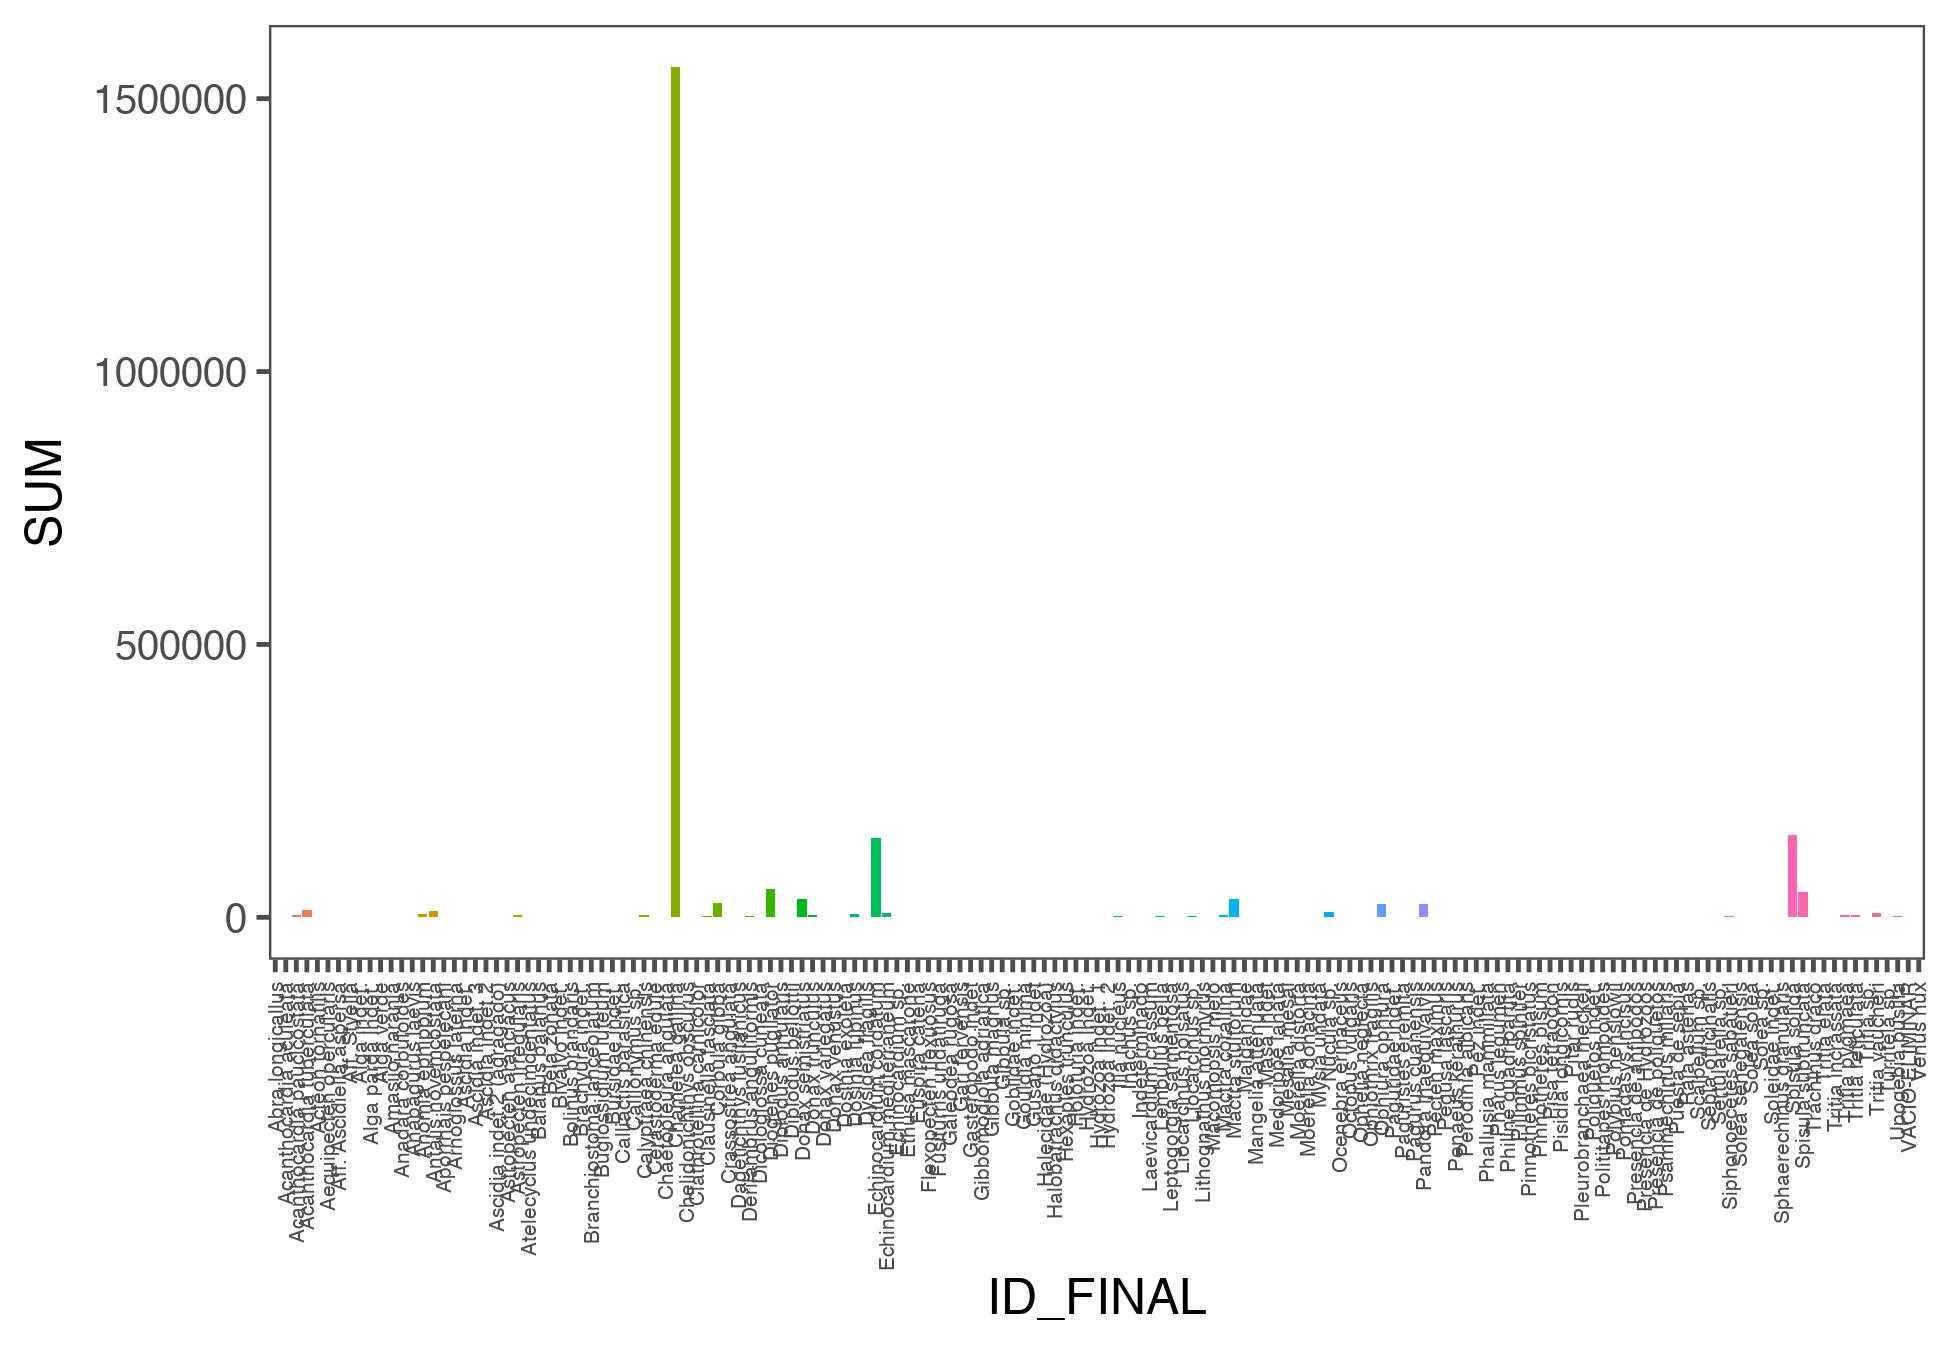
\includegraphics{SAR_Method_files/figure-latex/unnamed-chunk-4-1} \end{center}

\begin{center}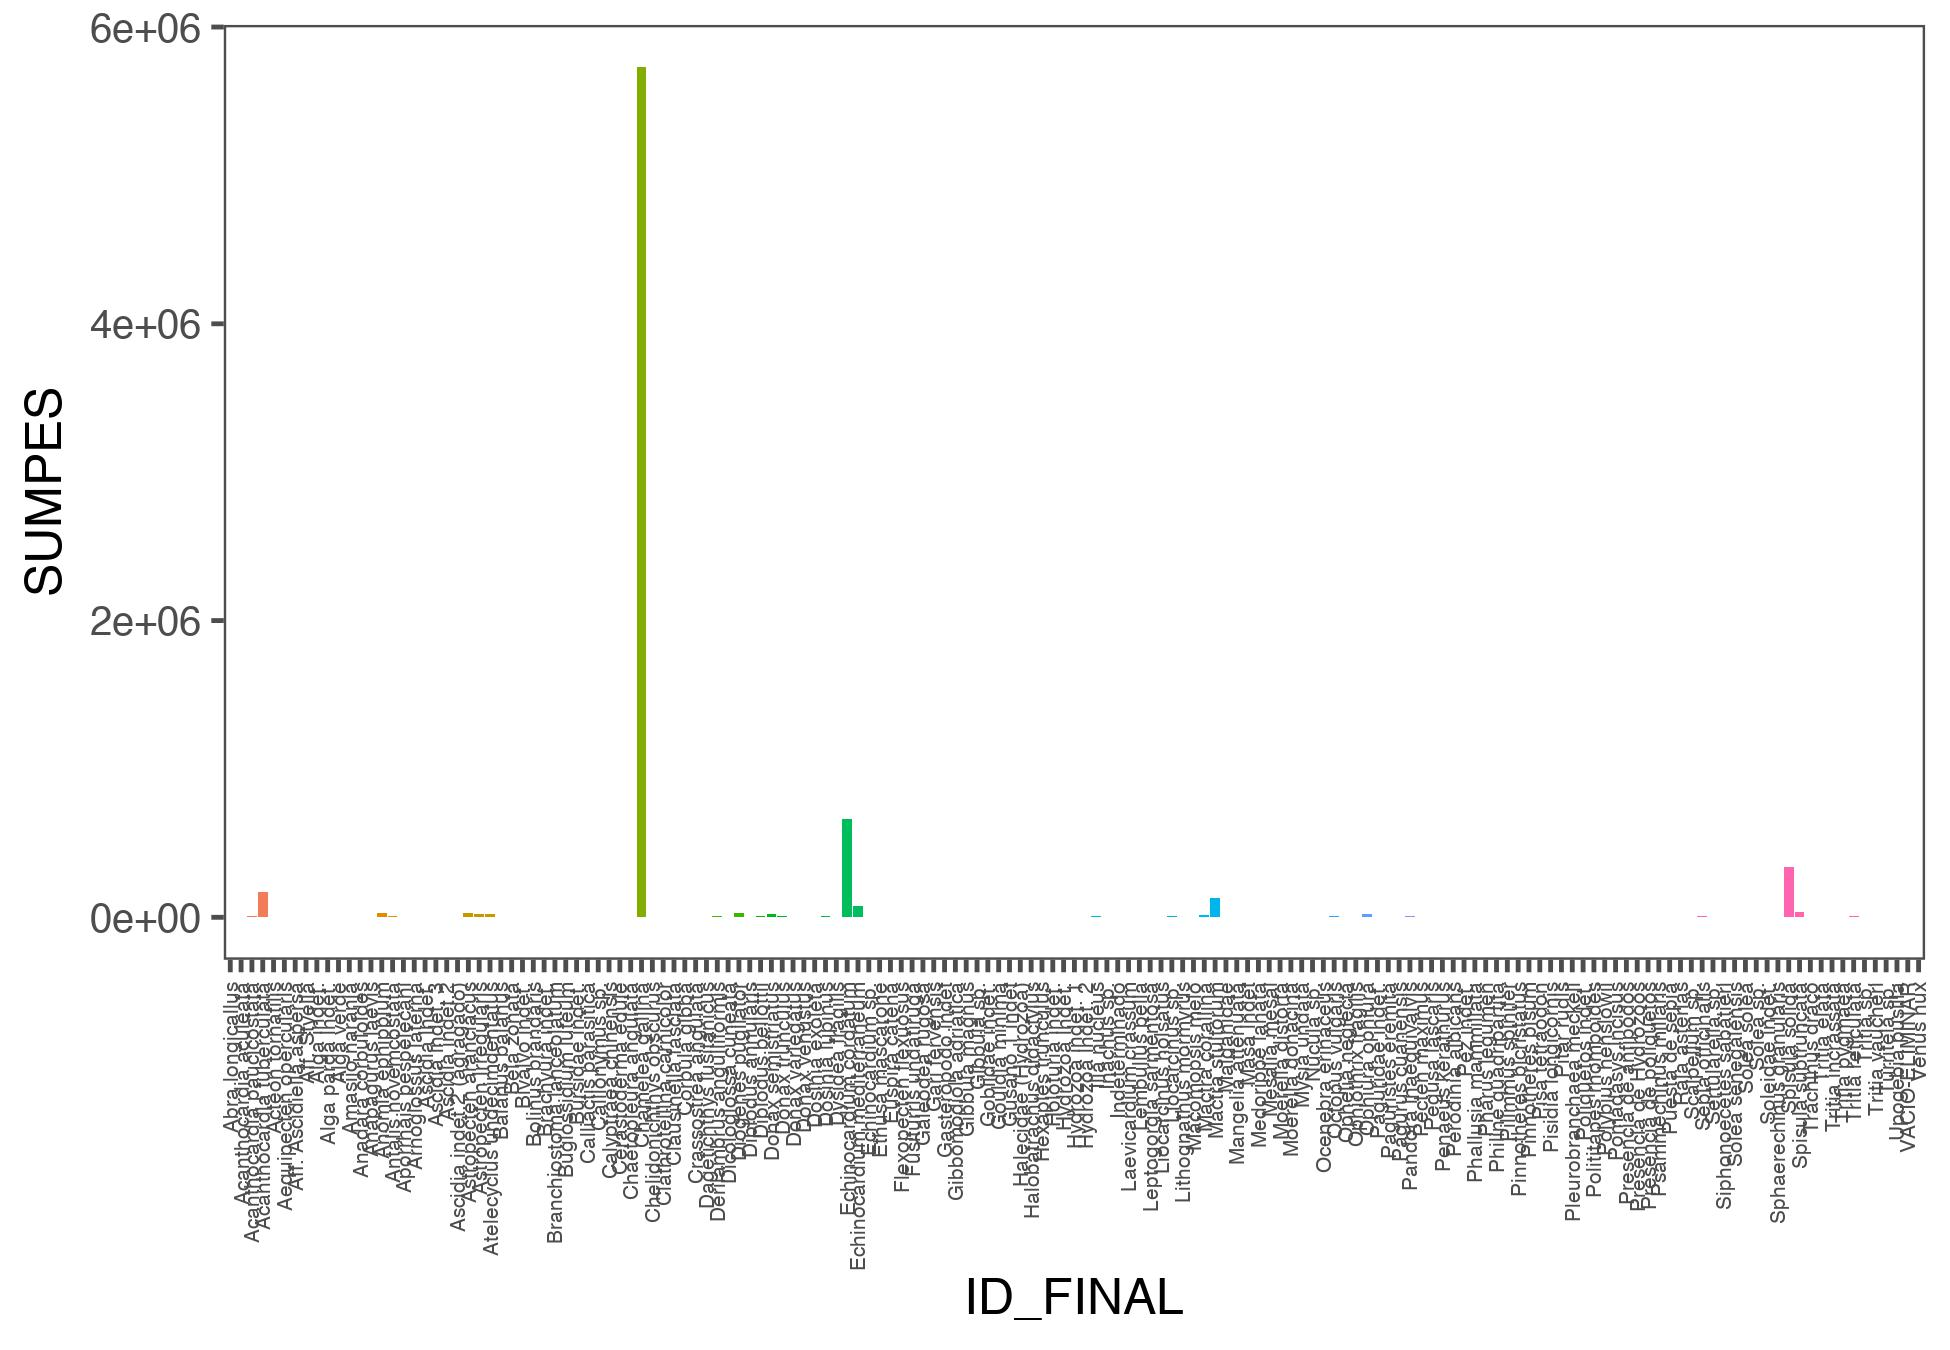
\includegraphics{SAR_Method_files/figure-latex/unnamed-chunk-5-1} \end{center}

\hypertarget{datos-lances}{%
\subsection{Datos Lances}\label{datos-lances}}

\begin{center}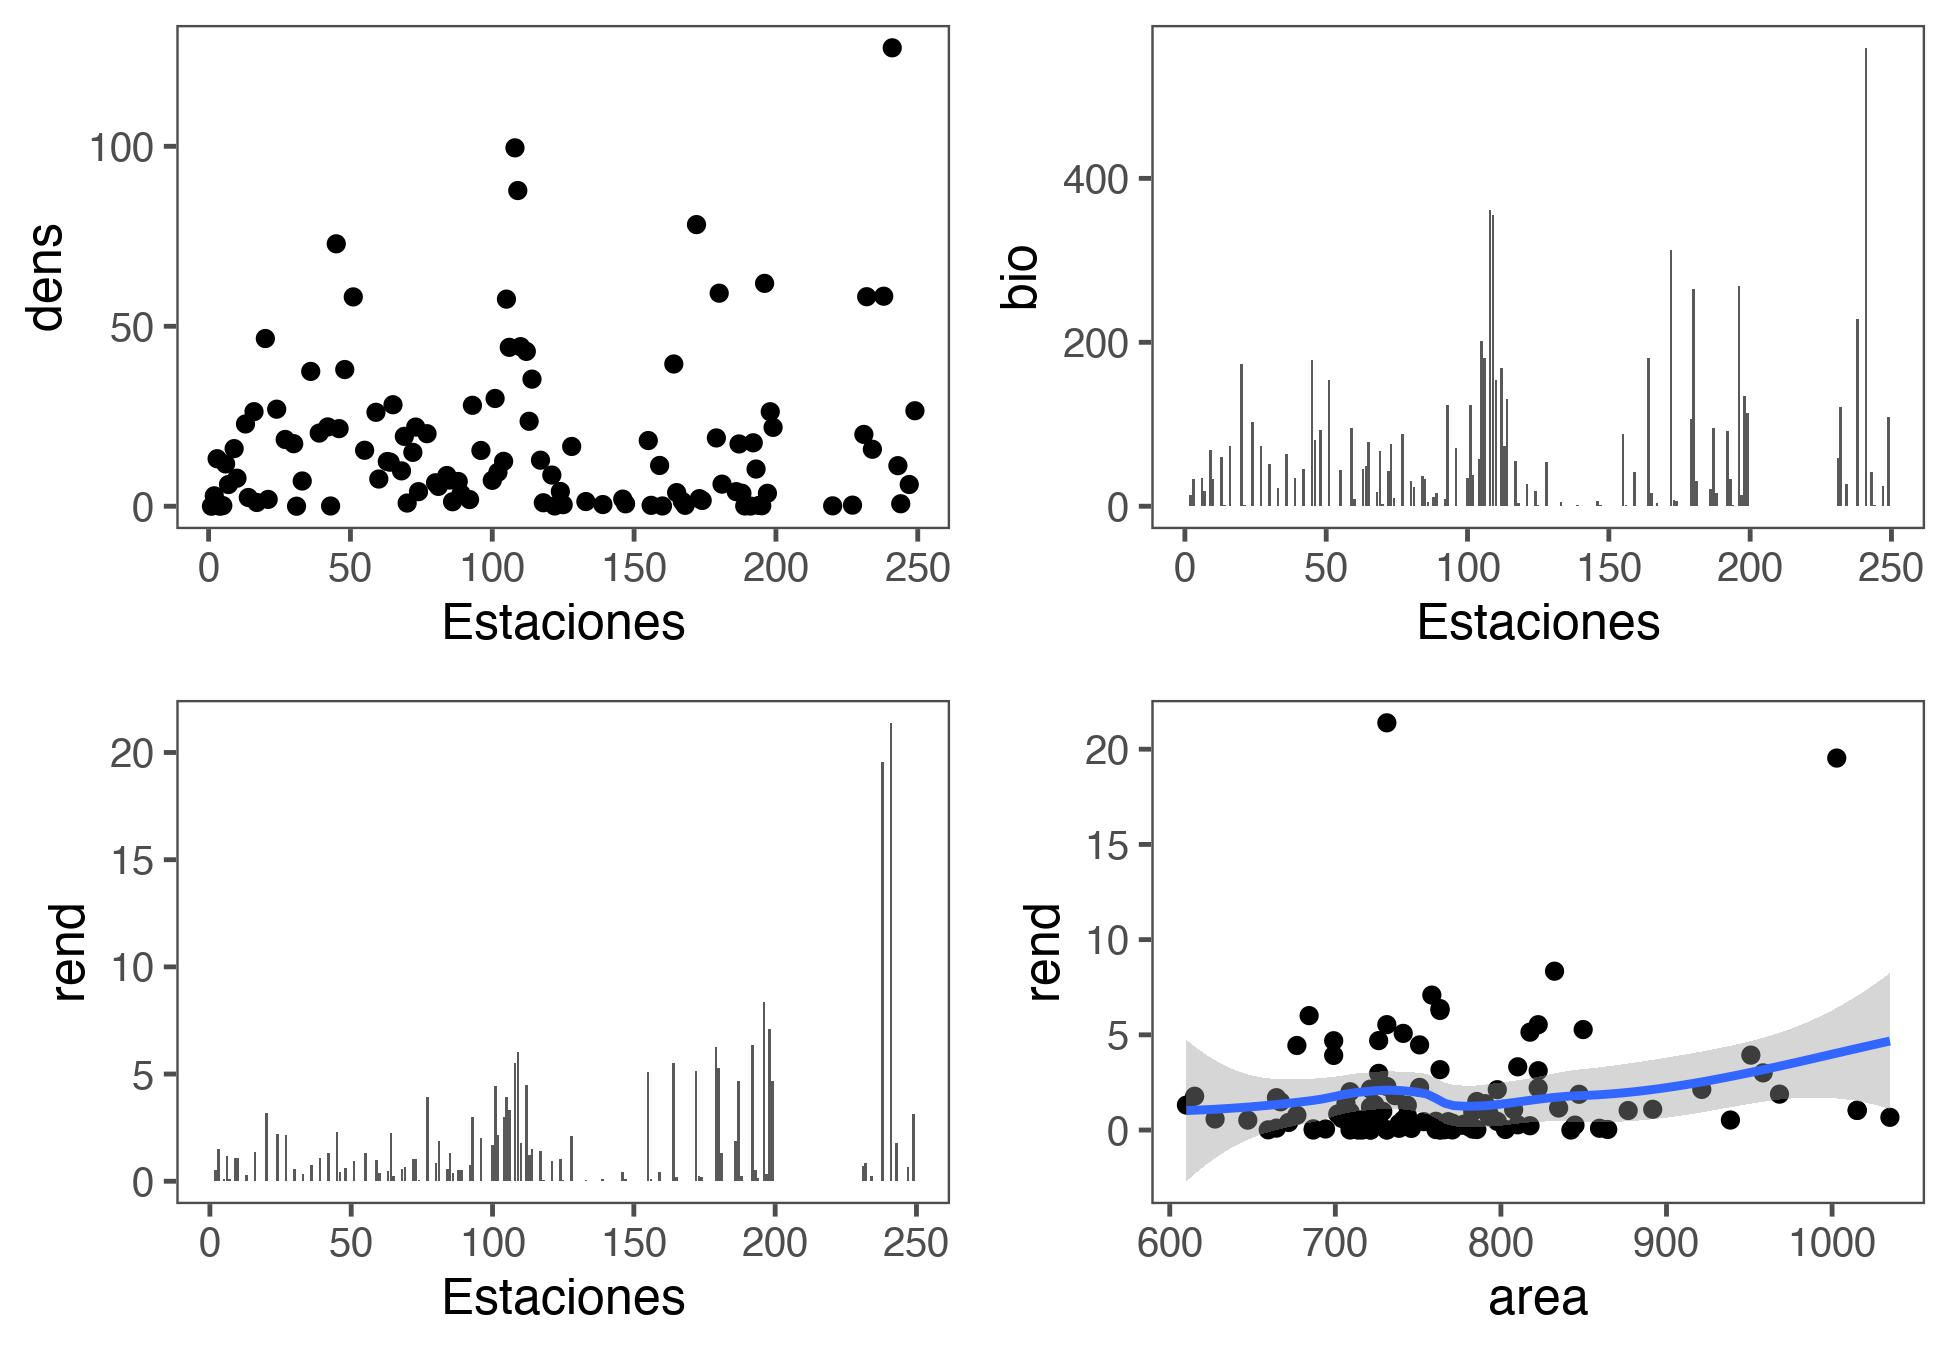
\includegraphics{SAR_Method_files/figure-latex/unnamed-chunk-6-1} \end{center}

Entender las profundidades

\begin{center}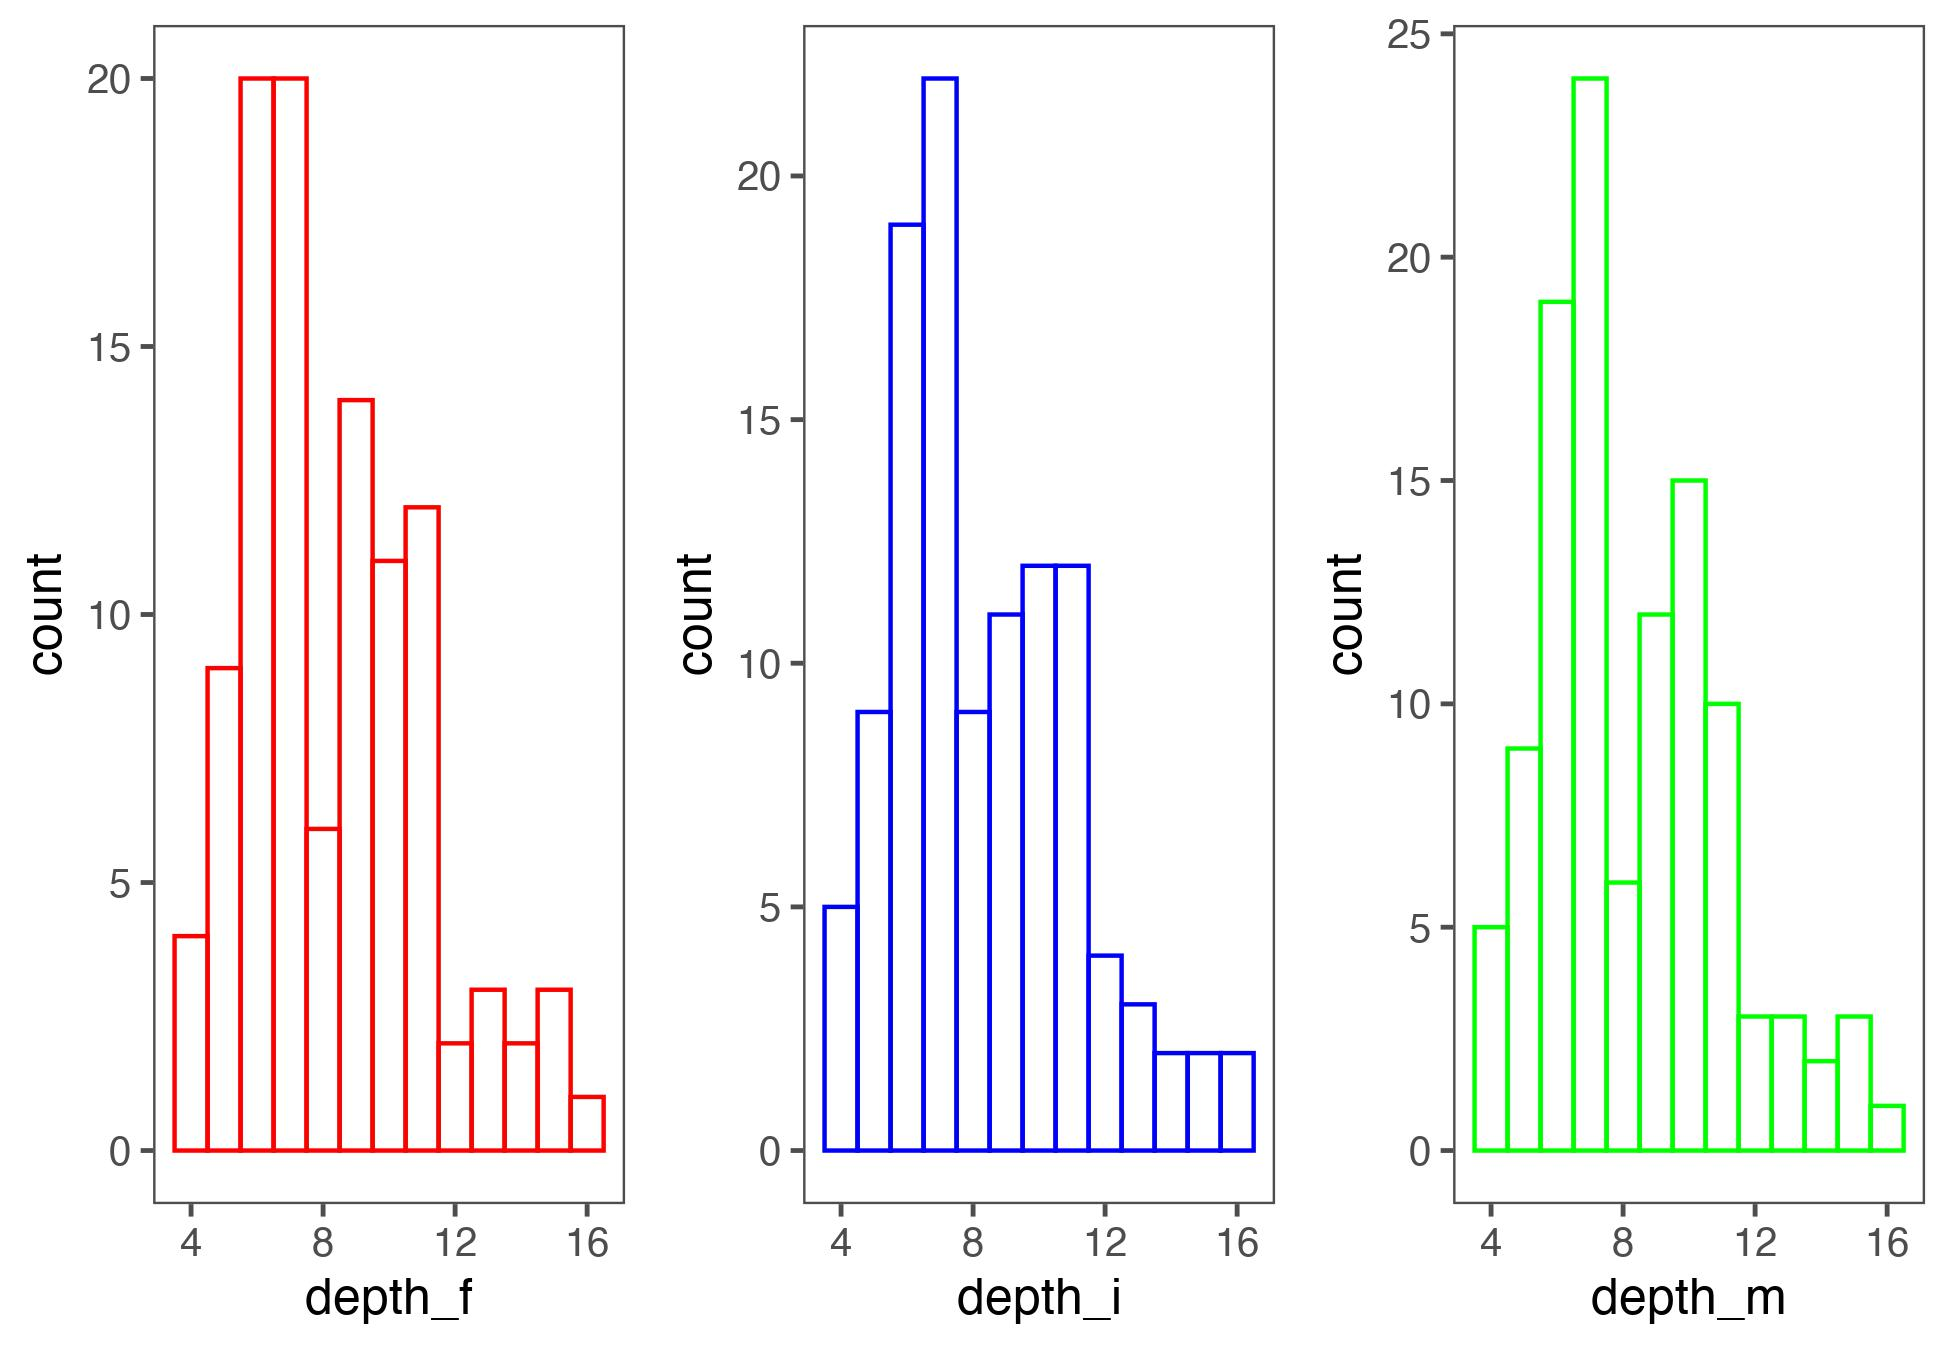
\includegraphics{SAR_Method_files/figure-latex/unnamed-chunk-7-1} \end{center}

\hypertarget{unir-bases}{%
\section{Unir bases}\label{unir-bases}}

\begin{verbatim}
##  [1] "CAMPAÑA"              "ESTACIÓN"             "CATEGORÍA"           
##  [4] "FECHA"                "PHYLA/Subphylum"      "GRUPO"               
##  [7] "ID_CAMPO"             "ID_FINAL"             "ESTACIÓN + CATEGORÍA"
## [10] "N_ DO...10"           "P_D0...11"            "N_D1...12"           
## [13] "P_D1...13"            "N_D2...14"            "P_D2...15"           
## [16] "N_D3...16"            "P_D3...17"            "Total Indiv...18"    
## [19] "Peso total (g)...19"  "N_ DO...20"           "P_D0...21"           
## [22] "N_D1...22"            "P_D1...23"            "N_D2...24"           
## [25] "P_D2...25"            "N_D3...26"            "P_D3...27"           
## [28] "Total Indiv...28"     "Peso total (g)...29"  "FP"                  
## [31] "N_ DO...31"           "P_D0...32"            "N_D1...33"           
## [34] "P_D1...34"            "N_D2...35"            "P_D2...36"           
## [37] "N_D3...37"            "P_D3...38"            "Total Indiv...39"    
## [40] "Peso total (g)...40"  "N_ DO...41"           "P_D0...42"           
## [43] "N_D1...43"            "P_D1...44"            "N_D2...45"           
## [46] "P_D2...46"            "N_D3...47"            "P_D3...48"           
## [49] "Total Indiv...49"     "Peso total (g)...50"  "%D0"                 
## [52] "%D1"                  "%D2"                  "%D3"                 
## [55] "%DT"
\end{verbatim}

\begin{verbatim}
## [1] "Estaciones"    "Observaciones" "area"          "station"
\end{verbatim}

\begin{verbatim}
##  [1] "Estaciones"              "Observaciones"          
##  [3] "Date"                    "Track"                  
##  [5] "Track (m)"               "depth_i"                
##  [7] "depth_f"                 "depth_m"                
##  [9] "vel_i"                   "vel_f"                  
## [11] "vel_m"                   "hora_i"                 
## [13] "hora_f"                  "g...14"                 
## [15] "min...15"                "g...16"                 
## [17] "min...17"                "LAT"                    
## [19] "LONG"                    "Nºrejillas"             
## [21] "Vol (l.)...21"           "Vol (l.)...22"          
## [23] "P (total + cascajo) (g)" "SW_tolva"               
## [25] "CSW"                     "CSW_tolva"              
## [27] "N"                       "N_tolva"                
## [29] "area"                    "dens"                   
## [31] "bio"                     "P cascajo (g)"          
## [33] "P cascajo_tolva"         "Tow_time"               
## [35] "PComercial (kg)"         "rend"                   
## [37] "ID"                      "FP"
\end{verbatim}

Cambio el nombre estación en \texttt{fauna}

\begin{Shaded}
\begin{Highlighting}[]
\NormalTok{fauna1 }\OtherTok{\textless{}{-}}\NormalTok{ fauna }\SpecialCharTok{\%\textgreater{}\%} 
  \FunctionTok{rename}\NormalTok{(}\StringTok{"Estaciones"}\OtherTok{=}\StringTok{"ESTACIÓN"}\NormalTok{) }\SpecialCharTok{\%\textgreater{}\%} 
  \FunctionTok{mutate}\NormalTok{(}\AttributeTok{Estaciones =} \FunctionTok{as.double}\NormalTok{(}\FunctionTok{str\_replace}\NormalTok{(Estaciones, }\StringTok{"\^{}E0*"}\NormalTok{, }\StringTok{""}\NormalTok{))) }\SpecialCharTok{\%\textgreater{}\%} 
  \FunctionTok{drop\_na}\NormalTok{(Estaciones)}
\end{Highlighting}
\end{Shaded}

\begin{Shaded}
\begin{Highlighting}[]
\NormalTok{base1  }\OtherTok{\textless{}{-}} \FunctionTok{left\_join}\NormalTok{(rendi, fauna1,}
                   \AttributeTok{by=}\StringTok{"Estaciones"}\NormalTok{)}
\end{Highlighting}
\end{Shaded}

\begin{Shaded}
\begin{Highlighting}[]
\FunctionTok{glimpse}\NormalTok{(base1)}
\end{Highlighting}
\end{Shaded}

\begin{verbatim}
## Rows: 2,119
## Columns: 92
## $ Estaciones                <dbl> 1, 1, 1, 1, 2, 2, 2, 2, 2, 2, 2, 2, 2, 2, 2,~
## $ Observaciones             <chr> NA, NA, NA, NA, NA, NA, NA, NA, NA, NA, NA, ~
## $ Date                      <dttm> 2019-05-06, 2019-05-06, 2019-05-06, 2019-05~
## $ Track                     <chr> ",\"P119-05-06 14:42:4", ",\"P119-05-06 14:4~
## $ `Track (m)`               <dbl> 278, 278, 278, 278, 380, 380, 380, 380, 380,~
## $ depth_i                   <dbl> 4.0, 4.0, 4.0, 4.0, 5.4, 5.4, 5.4, 5.4, 5.4,~
## $ depth_f                   <dbl> 4.0, 4.0, 4.0, 4.0, 3.6, 3.6, 3.6, 3.6, 3.6,~
## $ depth_m                   <dbl> 4.00, 4.00, 4.00, 4.00, 4.50, 4.50, 4.50, 4.~
## $ vel_i                     <dbl> 1.2, 1.2, 1.2, 1.2, 2.0, 2.0, 2.0, 2.0, 2.0,~
## $ vel_f                     <dbl> 1.2, 1.2, 1.2, 1.2, 1.7, 1.7, 1.7, 1.7, 1.7,~
## $ vel_m                     <dbl> 1.20, 1.20, 1.20, 1.20, 1.85, 1.85, 1.85, 1.~
## $ hora_i                    <dttm> 1899-12-31 14:37:17, 1899-12-31 14:37:17, 1~
## $ hora_f                    <dttm> 1899-12-31 14:42:45, 1899-12-31 14:42:45, 1~
## $ g...14                    <dbl> 37, 37, 37, 37, 37, 37, 37, 37, 37, 37, 37, ~
## $ min...15                  <dbl> 9.638, 9.638, 9.638, 9.638, 9.135, 9.135, 9.~
## $ g...16                    <dbl> 7, 7, 7, 7, 7, 7, 7, 7, 7, 7, 7, 7, 7, 7, 7,~
## $ min...17                  <dbl> 23.51, 23.51, 23.51, 23.51, 23.36, 23.36, 23~
## $ LAT                       <dbl> 37.16063, 37.16063, 37.16063, 37.16063, 37.1~
## $ LONG                      <dbl> 7.391833, 7.391833, 7.391833, 7.391833, 7.38~
## $ Nºrejillas                <dbl> 23.0, 23.0, 23.0, 23.0, 6.5, 6.5, 6.5, 6.5, ~
## $ `Vol (l.)...21`           <dbl> 354.19, 354.19, 354.19, 354.19, 97.40, 97.40~
## $ `Vol (l.)...22`           <dbl> 5, 5, 5, 5, 5, 5, 5, 5, 5, 5, 5, 5, 5, 5, 5,~
## $ `P (total + cascajo) (g)` <dbl> 3463.50, 3463.50, 3463.50, 3463.50, 3472.92,~
## $ SW_tolva                  <dbl> 245347.41, 245347.41, 245347.41, 245347.41, ~
## $ CSW                       <dbl> 0.00, 0.00, 0.00, 0.00, 661.76, 661.76, 661.~
## $ CSW_tolva                 <dbl> 0.00, 0.00, 0.00, 0.00, 12891.08, 12891.08, ~
## $ N                         <dbl> 0, 0, 0, 0, 139, 139, 139, 139, 139, 139, 13~
## $ N_tolva                   <dbl> 0.000, 0.000, 0.000, 0.000, 2707.720, 2707.7~
## $ area                      <dbl> 686.66, 686.66, 686.66, 686.66, 938.60, 938.~
## $ dens                      <dbl> 0.00000, 0.00000, 0.00000, 0.00000, 2.88485,~
## $ bio                       <dbl> 0.00000, 0.00000, 0.00000, 0.00000, 13.73438~
## $ `P cascajo (g)`           <lgl> NA, NA, NA, NA, NA, NA, NA, NA, NA, NA, NA, ~
## $ `P cascajo_tolva`         <lgl> NA, NA, NA, NA, NA, NA, NA, NA, NA, NA, NA, ~
## $ Tow_time                  <dttm> 1899-12-31 00:05:28, 1899-12-31 00:05:28, 1~
## $ `PComercial (kg)`         <dbl> 0.00000, 0.00000, 0.00000, 0.00000, 2.62219,~
## $ rend                      <dbl> 0.000000, 0.000000, 0.000000, 0.000000, 0.52~
## $ ID                        <dbl> 1, 1, 1, 1, 2, 2, 2, 2, 2, 2, 2, 2, 2, 2, 2,~
## $ FP.x                      <dbl> 70.838, 70.838, 70.838, 70.838, 19.480, 19.4~
## $ CAMPAÑA                   <chr> "ACUVEN-3D", "ACUVEN-3D", "ACUVEN-3D", "ACUV~
## $ CATEGORÍA                 <chr> "POBLACIONAL", "POBLACIONAL", "POBLACIONAL",~
## $ FECHA                     <dttm> 2019-05-06, 2019-05-06, 2019-05-06, 2019-05~
## $ `PHYLA/Subphylum`         <chr> "ANNELIDA", "ECHINODERMATA", "MOLLUSCA", "MO~
## $ GRUPO                     <chr> "POLYCHAETA", "ECHINOIDEA", "BIVALVIA", "BIV~
## $ ID_CAMPO                  <chr> "Poliquetos indet.", "Echinocardium mediterr~
## $ ID_FINAL                  <chr> "Ophelia neglecta", "Echinocardium mediterra~
## $ `ESTACIÓN + CATEGORÍA`    <chr> "E1", "E1", "E1", "E1", "E2", "E2-CAPTURA TO~
## $ `N_ DO...10`              <dbl> 1, 6, 14, 3, NA, NA, 2, 19, NA, 1, 73, NA, 2~
## $ P_D0...11                 <dbl> 0.290, 83.040, 38.540, 5.580, 9.190, NA, 2.7~
## $ N_D1...12                 <dbl> NA, NA, NA, NA, NA, NA, NA, NA, 2, NA, NA, N~
## $ P_D1...13                 <dbl> NA, NA, NA, NA, NA, NA, NA, NA, 9.24, NA, NA~
## $ N_D2...14                 <dbl> NA, NA, NA, NA, NA, NA, NA, NA, NA, NA, NA, ~
## $ P_D2...15                 <dbl> NA, NA, NA, NA, NA, NA, NA, NA, NA, NA, NA, ~
## $ N_D3...16                 <dbl> NA, 3, NA, NA, NA, NA, NA, NA, NA, NA, 107, ~
## $ P_D3...17                 <dbl> NA, 47.88, NA, NA, NA, NA, NA, NA, NA, NA, 9~
## $ `Total Indiv...18`        <dbl> 1, 9, 14, 3, 0, NA, 2, 19, 2, 1, 180, NA, 3,~
## $ `Peso total (g)...19`     <dbl> 0.290, 130.920, 38.540, 5.580, 9.190, NA, 2.~
## $ `N_ DO...20`              <dbl> NA, NA, NA, NA, NA, 1, NA, NA, NA, NA, NA, 1~
## $ P_D0...21                 <chr> NA, NA, NA, NA, NA, "249.34", NA, NA, NA, NA~
## $ N_D1...22                 <dbl> NA, NA, NA, NA, NA, NA, NA, NA, 1, NA, NA, N~
## $ P_D1...23                 <dbl> NA, NA, NA, NA, NA, NA, NA, NA, 4.34, NA, NA~
## $ N_D2...24                 <dbl> NA, NA, NA, NA, NA, NA, NA, NA, NA, NA, NA, ~
## $ P_D2...25                 <dbl> NA, NA, NA, NA, NA, NA, NA, NA, NA, NA, NA, ~
## $ N_D3...26                 <dbl> NA, NA, NA, NA, NA, NA, NA, NA, 1, NA, NA, N~
## $ P_D3...27                 <dbl> NA, NA, NA, NA, NA, NA, NA, NA, 6.35, NA, NA~
## $ `Total Indiv...28`        <dbl> NA, NA, NA, NA, NA, 1, NA, NA, 2, NA, NA, 1,~
## $ `Peso total (g)...29`     <dbl> NA, NA, NA, NA, NA, 249.34, NA, NA, 10.69, N~
## $ FP.y                      <dbl> 70.84, 70.84, 70.84, 70.84, 19.48, 19.48, 19~
## $ `N_ DO...31`              <dbl> 70.84, 425.04, 991.76, 212.52, 0.00, 0.00, 3~
## $ P_D0...32                 <dbl> 20.54360, 5882.55360, 2730.17360, 395.28720,~
## $ N_D1...33                 <dbl> 0.00, 0.00, 0.00, 0.00, 0.00, 0.00, 0.00, 0.~
## $ P_D1...34                 <dbl> 0.0000, 0.0000, 0.0000, 0.0000, 0.0000, 0.00~
## $ N_D2...35                 <dbl> 0, 0, 0, 0, 0, 0, 0, 0, 0, 0, 0, 0, 0, 0, 0,~
## $ P_D2...36                 <dbl> 0, 0, 0, 0, 0, 0, 0, 0, 0, 0, 0, 0, 0, 0, 0,~
## $ N_D3...37                 <dbl> 0.00, 212.52, 0.00, 0.00, 0.00, 0.00, 0.00, ~
## $ P_D3...38                 <dbl> 0.0000, 3391.8192, 0.0000, 0.0000, 0.0000, 0~
## $ `Total Indiv...39`        <dbl> 70.84, 637.56, 991.76, 212.52, 0.00, 0.00, 3~
## $ `Peso total (g)...40`     <dbl> 20.54360, 9274.37280, 2730.17360, 395.28720,~
## $ `N_ DO...41`              <dbl> 70.84, 425.04, 991.76, 212.52, 0.00, 1.00, 3~
## $ P_D0...42                 <dbl> 20.54360, 5882.55360, 2730.17360, 395.28720,~
## $ N_D1...43                 <dbl> 0.00, 0.00, 0.00, 0.00, 0.00, 0.00, 0.00, 0.~
## $ P_D1...44                 <dbl> 0.0000, 0.0000, 0.0000, 0.0000, 0.0000, 0.00~
## $ N_D2...45                 <dbl> 0, 0, 0, 0, 0, 0, 0, 0, 0, 0, 0, 0, 0, 0, 0,~
## $ P_D2...46                 <dbl> 0, 0, 0, 0, 0, 0, 0, 0, 0, 0, 0, 0, 0, 0, 0,~
## $ N_D3...47                 <dbl> 0.00, 212.52, 0.00, 0.00, 0.00, 0.00, 0.00, ~
## $ P_D3...48                 <dbl> 0.0000, 3391.8192, 0.0000, 0.0000, 0.0000, 0~
## $ `Total Indiv...49`        <dbl> 70.84, 637.56, 991.76, 212.52, 0.00, 1.00, 3~
## $ `Peso total (g)...50`     <dbl> 20.54360, 9274.37280, 2730.17360, 395.28720,~
## $ `%D0`                     <dbl> 100.00000, 66.66667, 100.00000, 100.00000, N~
## $ `%D1`                     <dbl> 0.00000, 0.00000, 0.00000, 0.00000, NA, 0.00~
## $ `%D2`                     <dbl> 0, 0, 0, 0, NA, 0, 0, 0, 0, 0, 0, 0, 0, 0, 0~
## $ `%D3`                     <dbl> 0.000000, 33.333333, 0.000000, 0.000000, NA,~
## $ `%DT`                     <dbl> 0.000000, 33.333333, 0.000000, 0.000000, NA,~
\end{verbatim}

\newpage

\hypertarget{referencias}{%
\section*{REFERENCIAS}\label{referencias}}
\addcontentsline{toc}{section}{REFERENCIAS}

\hypertarget{refs}{}
\begin{CSLReferences}{1}{0}
\leavevmode\vadjust pre{\hypertarget{ref-Indicator}{}}%
Indicator, C. (n.d.). \emph{{CEMP GUIDELINES FOR Common indicator Sentinels of the Seabed ( SoS )}} (pp. 1--38).

\end{CSLReferences}

\end{document}
